% This is a simple sample document.  For more complicated documents take a look in the exercise tab. Note that everything that comes after a % symbol is treated as comment and ignored when the code is compiled.

\documentclass{article} % \documentclass{} is the first command in any LaTeX code.  It is used to define what kind of document you are creating such as an article or a book, and begins the document preamble

\usepackage{amsmath} % \usepackage is a command that allows you to add functionality to your LaTeX code
\usepackage{datetime2}
\usepackage{calculo_comandos}
\usepackage{graphicx}
\usepackage{amssymb}
\usepackage{tikz}
\usepackage{pgfplots}
\usepackage{bm}
    \pgfplotsset{compat=newest}
\title{Simple Sample} % Sets article title
\author{My Name} % Sets authors name
\date{\today} % Sets date for date compiled
\graphicspath{{/workspaces/MAT-241/sources/img/}}

% The preamble ends with the command \begin{document}
\begin{document} % All begin commands must be paired with an end command somewhere
\maketitle % creates title using information in preamble (title, author, date)

\date{01-10-2024}
\section{Coordenadas no Espaço e Vetores no $R^3$} % creates a section
\subsection{Plano}

%grafico 1

\subsection{Espaço}

%regra da mão direita


Exemplo:
Localize no Espaço os pontos $P=(1,2,3)$ e $Q=(1,-2,3)$

%graficos

\subsection{Distancias entre pontos}

Exemplo:
$E \in R$, descreva os pontos dados pelas equações:
\begin{itemize}
     

\item[a.] $x=5$
\item[b.] $y =3$
\item[c.] $x^2 + y^2 = 1$
    $d((x,y)(0,0)) \rightarrow \sqrt{(x-0)^2 + (y-0)^2} = 1$ \\
    $\leftrightarrow \sqrt{x^2 + y^2} = 1 \leftrightarrow x^2 + y^2 = 1$ 

\end{itemize}

Exemplo: Que superficie em $R^3$ é representada pela seguinte equação?
\begin{itemize}
    \item[a.] $z=3$  \\ A equação $z=3$ representa o conjunto $\{(x,y,z) / z=3 \}$
    \item[b.] $y = 5$ \\ A equação $y=5$ representa um conjunto de todos os pontos do espaço que tem 2º coordenadas igual a 5.  
\end{itemize}

\subsubsection{Formula de Distancias}
\begin{figure}[!h]
    \centering
    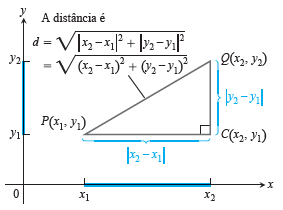
\includegraphics{graficodistancia.png}
    \caption{Descrição da imagem}
    \label{fig:exemplo}
\end{figure}
\date{03.10.2024}

Exemplo: Localize no $\mathbb{R}^2$ os pontos que satisfazem:
\begin{itemize}
    \item[a. ] $(x-1)^2 + (y-2)^2 = 1 $ e $z = 3$
    \item[b. ] $(x-4)(z-2) = 0$ 
        R: Note que $(x-4)(z-2) = 0$ ocorre $\leftrightarrow x -4 = 0$ ou $z-2=0 \leftrightarrow x = 4$ ou $z=2$             
\end{itemize}

Exemplo: Srjam P=(-5,2,3) e Q=(3,4,-1). Determine a esuqeção da esfera que tem $\overline{PQ}$ \\
Pmédio = $\left(\frac{x_1+x_2}{2}, \frac{y_1+y_2}{2}, \frac{z_1+z_2}{2} \right) $
%grafico 2d% \\
$P_u = u + \frac{1}{2}v = (x_1,y_1)+ \frac{1}{2}(x_2-x_1)(y_2 - y_1) = \left(\frac{x_2+x}{2} , \frac{y_2+y_1}{2} \right)$

\subsection{Vetores}
\textbf{Definição:}
Dados 2 pontos A ou B em $\mathbb{R}^3$ ou $\mathbb{R}^2$, o segmento orientado a $\overrightarrow{AB}$ é o segmento com ponto incicial A, ponto final V e orientado de $A \rightarrow B$.
%grafico 3%
\textbf{Definição:}
Um segmento não nulo de $\overrightarrow{AB}$ é equivalente a $\overrightarrow{CD}$ ou $\overrightarrow{AB}$ e $\overrightarrow{CD}$ tem o mesmo comprimento e direção e sentido %grafico acima%.
Dados dois segmentos orientados $\overrightarrow{AB}$ e $\overrightarrow{BC}$, definimos: a soma de $\overrightarrow{AB} + \overrightarrow{BC} = \overrightarrow{AC}$
Em geral, sejam u e v dois segmentos orientados. Para determina u+v, podemos seguir uma das duas abordagens:
\begin{figure}[!h]
    \centering
    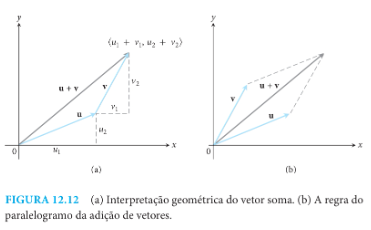
\includegraphics{graficosoma.png}
    \caption{Descrição da imagem}
    \label{fig:exemplo}
\end{figure}

Dado um segmento u de reta orientado $\overrightarrow{AB}$, existe um segmento de reta orientado $\overrightarrow{v}$, equiavalente a $\overrightarrow{AB}$ e com ponto inicial em (0,0,0). Para especificiar $\overrightarrow{v}$ precisamos apenas fornecer as coordenadas de um ponto final (a,b,c).
De modo geral, o vetor $\overrightarrow{v} = <x,y,z>$ é definido como o segmento de reta orientada com ponto inicial em (0,0,0) e ponto final $(x,y,z)$.


\textbf{Observação:} Sejam $u=<x,y,z>$ e $v=<x_2,y_2,z_2>$. Então: $u=v \leftrightarrow \{x_1 = x_2 \\ y_1 = y_2 \\ z_1 = z_2 \}$


\textbf{Observação:} Dados $A=(x_1,y_1,z_1)$ e $B=(x_2,y_2,z_2)$, o vetor equivalente a $\overrightarrow{AB}$ (ou vetor com representação $\overrightarrow{AB}$). $v = <x_2-x_1, y_2-y_1, z_2-z_1>$.


Exemplo: Dados $A=(1,4,0)$, $B=(-1,1,-1)$ e $C = (3,5,-10)$, encontre o vetor $\overrightarrow{v}$ equivalente a $\overrightarrow{AB}$ e as coordenadas do ponto D tal que $\overrightarrow{CD} = \overrightarrow{v}$
Solução: Segue se $v = <x_2-x_1, y_2-y_1, z_2-z_1>$ que $v=<-1-(1), 1-(4), -1-(0)> = <-2,-3,-1>$. Queremos encontrar D=(a,b,c) de tal modo que $\overrightarrow{v}$ seja equiavalente a $\overrightarrow{CD}$.
$<-2,-3,-1> = <a-3,b-5,c-(-10)> \leftrightarrow {a-3 = -2 \rightarrow a=1} {b-5 = -3 \rightarrow b=2} {c+10 = -1 \rightarrow c=-11}$ 

\subsubsection{Operação com Vetores}
\paragraph{Soma}: Sejam $\overrightarrow{u} = <x_1,y_1,z_1>$ e $\overrightarrow{v} = <x_2,y_2,z_2>$. Definimos a soma $\overrightarrow{u} + \overrightarrow{v}$ por $\overrightarrow{u} + \overrightarrow{v} = <x_1+x_2, y_1+y_2, z_1+z_2>$.
\paragraph{Produto Escalar}: Seja $k \in \mathbb{R}$ e $\overrightarrow{u} = <x_1,y_1,z_1>$. Definimos o produto $k*\overrightarrow{u} = <kx_1, ky_1, kz_1>$.
\paragraph{Comprimento}: O comprimento de $\overrightarrow{u} = <x_1, y_1, z_1>$ é $|| \overrightarrow{u} || = \sqrt{x_1^2, y_1^2, z_1^2}
\date{08-10-2024}

Exemplo: \mathexpr{\overrightarrow{u} = <4,0,3> e \overrightarrow{v} = <-2,1,5>}.
Determine: \\
\begin{itemize}
    \item[a.] \mathexpr{}
    \item[b. ]  
\end{itemize}

\subsubsection{Prorpiendades}: 

Sejam $\overrightarrow{u}, \overrightarrow{v}$ e $\overrightarrow{w}$ vetores do $\mathbb{R}$ e $a,b \in \mathbb{R}$.
Então: \\
\begin{itemize}
    \item[a.] $\overrightarrow{u} + \overrightarrow{v} = \overrightarrow{v} + \overrightarrow{u}$
    \item[b.] $(\overrightarrow{u}+ \overrightarrow{v}) + \overrightarrow{w} = \overrightarrow{u} + (\overrightarrow{v} + \overrightarrow{w})$  
    \item[c.] $\overrightarrow{u} + \overrightarrow{0} = \overrightarrow{u}$ 
    \item[d.] $\overrightarrow{u} + (-\overrightarrow{u}) = \overrightarrow{0}$ 
    \item[e.] $a (\overrightarrow{u} + \overrightarrow{v}) = a \overrightarrow{u} + a \overrightarrow{v}$
    \item[f.] $(a+b) \overrightarrow{u} = a \overrightarrow{u} + b \overrightarrow{u}$ 
    \item[g.] $(ab) \overrightarrow{u} = a (b \overrightarrow{u})$
    \item[h.] $1 \overrightarrow{u} = \overrightarrow{u}$ 
\end{itemize}

\subsubsection{Propriedades (Normas):}
\begin{itemize}
    \item[a.] $\norma{\overrightarrow{u}} \geq$ e $\norma{\overrightarrow{u}} = 0 \leftrightarrow \norma{u} = \norma{0}$
    \item[b.] $\norma{k \overrightarrow{u}} = |k| \norma{\overrightarrow{u}}$ 
    \item[c.] $ \|\vec{u} + \vec{v}\| \leq \|\vec{u}\| + \|\vec{v}\| \quad (\text{desigualdade do triângulo}$ 
\end{itemize}

$\text{Obs: Dado } \vec{u} = \vec{0}, \text{posso obter um novo vetor que é nulo.}$

\begin{align*}
    &\text{Temos } \vec{u} = \frac{\vec{u}}{\|\vec{u}\|}, \text{que} \\
    &\|\vec{u}\| = 1 \implies \|\lambda \vec{u}\| = \|\vec{u}\| = K \|\vec{u}\| \\
    &= 1 \implies K = \frac{1}{\|\vec{u}\|}
\end{align*}


Em $\mathbb{R}^3$, demonstremos por:
\begin{align*}
    \vec{i} &= \langle 1, 0, 0 \rangle \\
    \vec{j} &= \langle 0, 1, 0 \rangle \\
    \vec{k} &= \langle 0, 0, 1 \rangle
\end{align*}

Dai, seja $<x, y, z> \in \mathbb{R}^3$ então: TA ERRADO

$\langle \vec{x}, \vec{x} \rangle = x\langle \vec{e}_1, \vec{e}_1 \rangle + y\langle \vec{e}_1, \vec{e}_1 \rangle + z\langle \vec{e}_1, \vec{e}_1 \rangle$

$\vec{e}_i \in \{(1, 0, 0), (0, 1, 0), (0, 0, 1)\}$

$\Rightarrow \vec{x} \cdot \vec{x} = x^2 + y^2 + z^2$

Produto escalar

Def: Sejam $\vec{u} = (u_1, u_2, u_3)$ e $\vec{v} = (v_1, v_2, v_3)$. 

Definimos o produto escalar (interno)

$\vec{u} \cdot \vec{v} = u_1v_1 + u_2v_2 + u_3v_3$.
    

\date{22-10-2024}

\section{Plano no $R^3$}

3 pontos não colineares no espaço só definem um plano. Seja $\pi$ um plano no espaço, $P=(x_0, y_0, z_0)$ um ponto em
$\pi$ e $\overrightarrow{n} = < a,b,c >$ um vetor ortogonal a $\pi$. Isto é, $\overrightarrow{n} * \overrightarrow{QR} = 0$, quaisquer que sejam $Q$ e $R$ em $\pi$

%grafico 

Se $Q = (x,y,z)$ em $\pi$ então $\overrightarrow{PQ} = < x-x_0, y-y_0, z-z_0 >$ é ortogonal a $\overrightarrow{n}$, isto é: 

\begin{equation}\label{vetorial}
    < x- x_0, y- y_0, z - z_0 > * <a,b,c> = 0 \leftrightarrow a(x-x_0) + b(y-y_0) + c (z-z_0) = 0
\end{equation}
\eqref{vetorial} equação vetorial de $\pi$

Podemos então reescrever \eqref{vetorial} como: 
\begin{equation}\label{geral}
    ax + by + xz = ax_0 + by_0 + cz_0 -> d \leftrightarrow ax + by + cz = d
\end{equation}
\eqref{geral} equação geral de $\pi$

\paragraph{Exemplo:}
Escreva a equação do plano que contém $P = (1,1,-2)$, $Q = (0,2,1)$ e $R = (-1,-1,0)$

%grafico

Para determinar um vetor ortogonal ao plano, basta tomar o produto vetorial $\overrightarrow{n} = \overrightarrow{PQ} * \overrightarrow{PR} = <-1,1,3> * <-2,-2,2>$

\[
\begin{vmatrix}
    \hat{i} & \hat{j} & \hat{k} \\ 
    -1 & 1 & 3 \\ 
    -2 & -2 & 2 
\end{vmatrix}
\] = $<8,-4,4>$

Daí, a equação vetorial do plano que contem P, Q e R é: $8(x-1) - 4(y-1) + 4(z+2) = 0$.
A equação geral é $8x-4y+4z = 8-4-8 = -4 \leftrightarrow 8x - 4y + 8z = -4$

\paragraph{Exemplo:} Somente a equação do plano que passa por $(1,4,3)$ e contém a reta:
\begin{equation}
    x = \frac{y-1}{2} = z+1 
\end{equation}

\paragraph{1º Solução:} Percebe que $P=(1,4,3)$, $Q=(0,1,-1)$ e $R = (1,3,0)$ pertecem ao plano $\pi$. 

\subsection{Distnacia entre um ponto e um plano}

Trocando po P uma reta paralela ao vetor normal, $(\overrightarrow{n})$ ao plano e denotando por R o ponto onde tal reta interecepta o plano $\pi$, definindo a distância de P em $\pi$ por:
$d = || \overrightarrow{RP} || = || P-R || $

Assim, 
$d = || Proj_{\overrightarrow{n} \overrightarrow{PQ}}$
%
\textbf{Hello World!} Today I am learning \LaTeX. %notice how the command will end at the first non-alphabet charecter such as the . after \LaTeX
\LaTeX{} is a great program for writing math. I can write in line math such as $a^2+b^2=c^2$ %$ tells LaTexX to compile as math
. I can also give equations their own space:
\begin{equation} % Creates an equation environment and is compiled as math
  \gamma^2+\theta^2=\omega^2
\end{equation}
If I do not leave any blank lines \LaTeX{} will continue  this text without making it into a new paragraph.  Notice how there was no indentation in the text after equation (1).
Also notice how even though I hit enter after that sentence and here $\downarrow$
\LaTeX{} formats the sentence without any break.  Also   look  how      it   doesn't     matter          how    many  spaces     I put     between       my    words.
%
For a new essay I can leave a blank space in my code.

\end{document} % This is the end of the document